\documentclass{utmreport}
\selectlanguage{english}
\ifPDFTeX\else\setmonofont{Liberation Mono}\fi
\utmlogo{assets/UTM_Logo_English.jpeg}
\institution{Technical University of Moldova}
\faculty{Faculty of Computers, Informatics, and Microelectronics}
\department{Department of Software Engineering}
\studyprogramme{Software Engineering Study Programme}
\documenttype{Laboratory report no. 1}
\reporttitle{Caesar Cipher over the Romanian Alphabet}
\reportsubtitle{C++ implementation with custom UTF-8 and UTF-32 conversion}
\cityyear{Chișinău}{2026}
% Author, group, supervisor and repository used by main.tex.
\student{Gabriel Balan}{FAF-241}
\supervisor{asist. univ. Zaica Maia}{}
\newcommand{\repositoryurl}{https://github.com/AverageCEnj0yer/Cryptography}

% Unicode-safe verbatim rendering preserves Romanian code points in excerpts.
\usepackage{fvextra}
\fvset{fontfamily=tt,fontsize=\footnotesize,baselinestretch=1,
       breaklines=true,breakanywhere=true}
\newcommand{\sourceexcerpt}[2]{\VerbatimInput[firstline=#1,lastline=#2]{../src/main.cpp}}
\DefineVerbatimEnvironment{cppcode}{Verbatim}{}
\DefineVerbatimEnvironment{console}{Verbatim}{fontsize=\footnotesize}
\setlength{\emergencystretch}{2em}
\begin{document}
\makeutmreporttitlepage
\tableofcontents
\clearpage
\begin{utmabstract}[Abstract]
This laboratory implements the standard Caesar cipher and its keyword-permuted variant for the 31-letter Romanian alphabet in C++. Beyond the substitution itself, the implementation includes a custom bidirectional UTF-8/UTF-32 conversion layer. It decodes variable-length byte sequences, checks their structure and scalar-value ranges, processes complete Unicode code points, and encodes results back into terminal-compatible UTF-8. Romanian case conversion and cedilla compatibility are implemented explicitly, while cipher arithmetic uses alphabet positions rather than Unicode values. The report explains these design decisions, presents the supplied terminal screenshots, and distinguishes the encryption interface from the decryption functionality available in the underlying functions. Supplementary checks verify both directions and the encoding boundaries without modifying the application source.

\utmkeywords{Caesar cipher, C++, UTF-8, UTF-32, Romanian alphabet, bit masks, input validation}
\end{utmabstract}

\utmintroduction
The objective of Laboratory Work No. 1 is to implement and understand two Caesar cipher variants using the Romanian alphabet specified in the handout \cite{handout}. The numeric key belongs to $\{1,\ldots,30\}$; the second variant also uses a keyword of at least seven letters to reorder the alphabet. The exercise combines modular arithmetic, text normalization, validation, and an evaluation of the ciphers' security.

The implementation is contained in \texttt{Lab\_1/src/main.cpp} \cite{implementation}. Its CMake configuration requests C++23 and builds the executable \texttt{lab1} with strict compiler warnings. It uses the C++ standard library without an external Unicode library. The project extends the cipher exercise into a study of character encoding: instead of treating a terminal string as a sequence of single-byte letters, it explicitly converts between UTF-8 and UTF-32.

This separation matters for Romanian diacritics. A character such as Ș occupies two bytes in UTF-8 but must occupy one position in the cipher alphabet. The conversion functions also handle three- and four-byte sequences, allowing the application to distinguish valid Unicode outside the Romanian alphabet from malformed encoding. The report follows the actual source: the command-line argument selects one or two keys, while a Boolean function parameter controls decryption internally.

\chapter{Short theory}
\section{Standard Caesar cipher}
The Romanian alphabet has $n=31$ letters in this fixed order:
\begin{center}\texttt{AĂÂBCDEFGHIÎJKLMNOPQRSȘTȚUVWXYZ}.\end{center}
Its indices are $A=0$, $\text{Ă}=1$, $\text{Â}=2$, $B=3$, and so on through $Z=30$. If $x$ is the plaintext letter's index and $y$ is the ciphertext letter's index, then
\begin{equation}
E_k(x)=(x+k)\bmod31,\qquad D_k(y)=(y+31-k)\bmod31.
\end{equation}
Adding 31 in decryption keeps the intermediate value nonnegative for an allowed key. The modulo operation wraps past the ends of the alphabet: with $k=1$, $Z$ encrypts to $A$, and $A$ decrypts to $Z$.

The key space contains only 30 shifts, making exhaustive search practical. Uppercasing and deleting spaces are preprocessing operations; decryption recovers the normalized letter sequence, not the original capitalization or word boundaries.

\section{Caesar cipher with a keyword permutation}
The second key is a sequence of at least seven Romanian letters. Its first occurrences are written in order, followed by all unused letters of the natural alphabet. For the keyword \texttt{UCRAINA}, the repeated $A$ is discarded during construction, producing
\begin{center}\texttt{UCRAINĂÂBDEFGHÎJKLMOPQSȘTȚVWXYZ}.\end{center}
The keyword has seven letters before deduplication and contributes six distinct letters. The length rule therefore does not require seven distinct letters.

If $P$ denotes the resulting ordered alphabet and $\operatorname{pos}_P(a)$ is the position of letter $a$ in it, the transformations are
\begin{align}
E_{k,P}(a)&=P[(\operatorname{pos}_P(a)+k)\bmod31],\\
D_{k,P}(a)&=P[(\operatorname{pos}_P(a)+31-k)\bmod31].
\end{align}
Both lookup and output indexing use $P$. A lookup in the original alphabet followed by output from $P$ would define a different transformation.

Allowing arbitrary keywords makes all $31!$ alphabet orderings attainable, so the nominal number of alphabet--shift pairs is
\begin{equation}
30\cdot31!\approx2.47\cdot10^{35}.
\end{equation}
These pairs are not all distinct encryptions. Since 31 is prime, every nonzero shift visits all 31 positions before returning to its starting point. Reordering the alphabet relabels this cycle; consequently the distinct substitutions are the $30!$ possible cycles containing all 31 letters. This is still a monoalphabetic cipher: each occurrence of a given letter receives the same replacement. Letter frequencies and repeated-letter patterns remain available to an attacker, despite the much larger nominal key space.

\chapter{Implementation}
\section{Representation and processing stages}
The program uses three distinct notions of a character: UTF-8 bytes at the input/output boundary, Unicode code points in \texttt{std::u32string}, and indices from 0 to 30 for the cipher. The processing sequence is
\begin{center}
\small
UTF-8 input $\longrightarrow$ UTF-32 decoding $\longrightarrow$ normalization\\
$\longrightarrow$ alphabet validation $\longrightarrow$ index-based substitution\\
$\longrightarrow$ UTF-8 encoding $\longrightarrow$ terminal output.
\end{center}
Unicode values determine how a character is represented and recognized; they never determine its Caesar displacement. The alphabet constants provide the laboratory's required encoding directly:
\sourceexcerpt{12}{14}
The \texttt{U} prefix creates UTF-32 literals. The two \texttt{constexpr std::u32string\_view} objects refer to fixed uppercase and lowercase alphabets without owning a dynamically allocated copy. Their matching positions make Romanian case conversion independent of the terminal locale. \texttt{std::string\_view} and \texttt{std::u32string\_view} also let functions inspect existing strings without copying the input just to pass it as an argument; conversion outputs still own their storage.

\section{Custom UTF-8 to UTF-32 decoder}
\subsection{Recognizing a sequence and reconstructing a code point}
\texttt{utf8\_to\_utf32} advances a byte index through the input. The leading byte is converted to \texttt{unsigned char}, so high-bit byte values are processed as nonnegative values even on platforms where plain \texttt{char} is signed. Its leading bits identify the number of bytes:

\begin{table}[htbp]
\centering
\caption{UTF-8 sequence structure handled by the decoder}
\begin{tabular}{c l l}
\hline
Bytes & Bit pattern & Scalar-value range\\
\hline
1 & \texttt{0xxxxxxx} & \texttt{U+0000--U+007F}\\
2 & \texttt{110xxxxx 10xxxxxx} & \texttt{U+0080--U+07FF}\\
3 & \texttt{1110xxxx 10xxxxxx 10xxxxxx} & \texttt{U+0800--U+FFFF}*\\
4 & \texttt{11110xxx 10xxxxxx 10xxxxxx 10xxxxxx} & \texttt{U+10000--U+10FFFF}\\
\hline
\end{tabular}
\par\smallskip\footnotesize *Excluding the surrogate range \texttt{U+D800--U+DFFF}.
\end{table}

For a two-byte sequence, \texttt{(b1 \& 0xE0) == 0xC0} recognizes the \texttt{110} prefix. The expression \texttt{(b2 \& 0xC0) == 0x80} checks that the next byte starts with \texttt{10}. After those checks, the payload bits are combined:
\sourceexcerpt{38}{38}
The first mask keeps five payload bits, shifting them left by six positions; the second keeps six bits. Bitwise OR joins them into an 11-bit value. For example, Ș is \texttt{U+0218}, encoded as bytes \texttt{C8 98}:
\begin{equation}
((\mathtt{C8}\mathbin{\&}\mathtt{1F})\ll6)
\mathbin{|}(\mathtt{98}\mathbin{\&}\mathtt{3F})
=(8\cdot64)+24=536=\mathtt{0x0218}.
\end{equation}
The same idea extends to three bytes with shifts of 12 and 6, and four bytes with shifts of 18, 12 and 6:
\sourceexcerpt{78}{81}
Each decoded value is appended once to the UTF-32 output. Romanian letters then occupy one string element each, and indexing cannot accidentally select half of a multibyte letter.

\subsection{Structural and scalar-value validation}
The decoder checks that enough bytes remain before reading a multibyte sequence, then validates every continuation-byte prefix. It also checks the reconstructed value against the range appropriate to that sequence length. These are separate checks: a sequence can have the correct prefixes while representing an invalid value.

The minimum values \texttt{0x80}, \texttt{0x800}, and \texttt{0x10000} reject overlong encodings, where a value is written using more bytes than necessary. The three-byte branch rejects surrogate code points, which are reserved for UTF-16 and are not Unicode scalar values. The four-byte branch rejects values greater than \texttt{0x10FFFF}. Unexpected leading bytes, isolated continuation bytes, and incomplete sequences reach an error path. Structural failures terminate with status 1; the decoder's reconstructed-value range failures terminate with status 2.

This creates a useful distinction. A valid four-byte emoji can be decoded correctly and subsequently rejected by the Romanian alphabet validator, with the whole character printed in the diagnostic. A malformed byte sequence cannot first become a valid internal character and causes immediate termination. The conversion layer understands a broader set of characters than the cipher permits.

\section{Custom UTF-32 to UTF-8 encoder}
\texttt{utf32\_to\_utf8} performs the reverse operation. It selects one, two, three or four output bytes according to the scalar value, explicitly rejecting surrogate values and values above \texttt{U+10FFFF}. Payload bits are extracted with right shifts and masks; fixed prefix bits are added with bitwise OR. The two-byte case is:
\sourceexcerpt{135}{138}
The continuation byte receives its \texttt{10} prefix from \texttt{0x80}; the leading byte receives \texttt{110} from \texttt{0xC0}. Although the continuation byte is calculated first, the leading byte is appended first, preserving the required byte order. The three- and four-byte cases use the same construction with additional six-bit groups.

Encoding is necessary for more than the final ciphertext. When validation finds an unsupported code point, the program creates a one-element \texttt{std::u32string} and converts it back to UTF-8 for the error message. This is why the screenshot can identify a Hebrew letter or an emoji as a complete character instead of displaying an individual byte. The functions operate on code points; they do not segment user-perceived grapheme clusters or perform general Unicode normalization.

\section{Romanian normalization and message validation}
The \texttt{normalize} function first maps the historical cedilla variants to the modern comma-below forms, then converts lowercase letters using their position in the lowercase alphabet:
\sourceexcerpt{216}{231}
Thus \texttt{ş}, \texttt{Ş}, \texttt{ș}, and \texttt{Ș} become the same uppercase letter. Romanian diacritics remain distinct alphabet entries: Ă and  do not become $A$, and Î does not become $I$. This preserves the specified 31-letter encoding.

The message validator decodes and normalizes the string, then searches for the first character that is neither a Romanian letter nor an ordinary space:
\sourceexcerpt{240}{243}
When such a character is found, it is encoded back to UTF-8 and reported; \texttt{getMessage} requests a new message. If validation succeeds, the caller's string is replaced with its normalized UTF-8 representation. Both cipher functions repeat normalization and alphabet checks internally, so direct calls do not depend on the interactive validator having run first.

Only \texttt{U+0020} is accepted as an internal message space and erased before transformation. The input expression \texttt{std::getline(std::cin >> std::ws, message)} consumes leading whitespace, including blank lines, before reading a line; it does not make internal tabs valid. No NFC composition is implemented: a precomposed ă is accepted, while $a$ followed by a separate combining breve is rejected at the combining mark. Here ``normalization'' means the explicit Romanian mappings above.

\section{Numeric input and command-line control}
\texttt{getInt} reads an integer and marks the stream as failed if it is outside 1--30:
\sourceexcerpt{194}{198}
The helper \texttt{clearFailedExtraction} handles extraction errors and leftover characters. It clears the stream state and discards the rest of the line before the next attempt. Consequently inputs such as \texttt{6abc} and \texttt{6.5} are rejected rather than silently becoming the key 6. The leftover-input check is strict: even a space after an otherwise valid number is rejected. Numeric end-of-input handling exits when the helper detects EOF.

The program is invoked as \texttt{./build/lab1 1} for the standard cipher or \texttt{./build/lab1 2} for the keyword variant. \texttt{main} checks the argument count before accessing \texttt{argv[1]}, and catches exceptions from \texttt{std::stoi}. The \texttt{begin} function then reads the message and shift, and uses a switch to select the variant; mode 2 additionally requests a keyword. The run ends after one operation.

Argument parsing is distinct from numeric-key validation: \texttt{std::stoi} is called without checking the number of consumed characters, so a prefix such as \texttt{1abc} can be interpreted as mode 1. Numeric modes other than 1 or 2 reach the switch's diagnostic after message and key input. The supplied multi-argument screenshot exercises the argument-count check specifically.

\section{Constructing and validating the permuted alphabet}
The keyword is decoded and normalized before its length is examined:
\sourceexcerpt{335}{344}
Because \texttt{keyword32.size()} counts code points, four two-byte Romanian letters cannot incorrectly satisfy a seven-letter requirement merely by occupying eight UTF-8 bytes. A subsequent loop rejects any character outside the Romanian alphabet, including an internal space. Invalid keywords print a diagnostic and terminate with status 1; there is no keyword retry loop.

The alphabet is constructed in two passes:
\sourceexcerpt{361}{376}
The first pass preserves the order of distinct keyword letters. The second supplies every missing Romanian letter in the required order. A letter is appended only if it is absent, so the completed alphabet contains all 31 letters exactly once. \texttt{reserve} allocates capacity for that known size without adding characters. The alphabet is printed after construction, making the second key's effect directly inspectable.

For \texttt{cryptographieeee}, the uppercase keyword contributes \texttt{CRYPTOGAHIE}. Repeated occurrences of $R$, $P$, and $E$ do not create extra entries. The final alphabet is
\begin{center}\texttt{CRYPTOGAHIEĂÂBDFÎJKLMNQSȘȚUVWXZ}.\end{center}
A longer keyword therefore need not produce a different alphabet or a stronger substitution; first-occurrence order is what determines the permutation.

\section{Encryption, decryption and wraparound}
Both cipher functions decode and normalize the message. They remove ordinary spaces with \texttt{std::erase} and reserve output capacity equal to the remaining number of code points. For each letter, \texttt{find} returns its position in the active alphabet. A failed lookup causes a diagnostic instead of allowing \texttt{npos} to enter the arithmetic. The standard version then applies:
\sourceexcerpt{305}{322}
The decryption branch adds the alphabet length before subtracting the key. This is particularly relevant because \texttt{pos} and \texttt{newPos} use the unsigned type \texttt{std::size\_t}. With $1\le k\le30$, the intermediate value cannot underflow. The permuted version uses identical arithmetic with \texttt{permuted.find(c)} and \texttt{permuted.size()}.

Both functions expose \texttt{bool decrypt = false}; passing \texttt{true} selects the inverse transformation. However, \texttt{begin} calls them without this argument, so the current interactive interface performs encryption only. Numeric-key validation belongs to \texttt{getInt}; callers using the cipher functions directly must also respect the 1--30 precondition.

For a message of $m$ code points and a keyword of $q$ code points, alphabet searches inspect at most 31 entries. Transformation therefore takes $O(31m)$ time and permutation construction $O(31q+31^2)$, both linear in input length for this fixed alphabet. The strings require linear storage. UTF-32 makes processing straightforward at the cost of four bytes per code unit; the application also performs some repeated conversions between its validation and cipher stages. The design favors explicit, inspectable steps over minimizing every allocation.

\chapter{Results}
\section{Standard and keyword-based encryption}
Figure~\ref{fig:successful} is the supplied screenshot of two runs of the C++ executable. Both use the plaintext ``Trimite două sute de mii de soldați să cucerească Moldova''. After uppercasing and removing spaces, the 48-letter message is:
\begin{console}
TRIMITEDOUĂSUTEDEMIIDESOLDAȚISĂCUCEREASCĂMOLDOVA
\end{console}
For the standard alphabet and $k=6$, the result is:
\begin{console}
YVNSNYJÎTAFWAYJÎJSNNÎJWTRÎEZNWFIAIJVJEWIFSTRÎTĂE
\end{console}
For example, $T$ has index 23 and becomes the letter at $(23+6)\bmod31=29$, namely $Y$. Likewise, $R$ at index 20 becomes $V$ at index 26.

For $k=8$ and keyword \texttt{UCRAINA}, the program prints the new alphabet and ciphertext:
\begin{console}
UCRAINĂÂBDEFGHÎJKLMOPQSȘTȚVWXYZ
CEGVGCMLWBÎZBCMLMVGGLMZWȚLFRGZÎDBDMEMFZDÎVWȚLWAF
\end{console}
In this alphabet $T$ has index 24, so it maps to index $(24+8)\bmod31=1$, which contains $C$. The changed ordering therefore explains why the two ciphertexts begin differently.

\begin{figure}[htbp]
\centering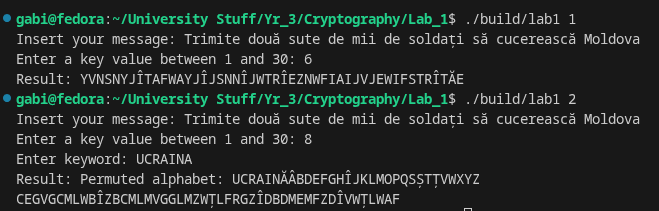
\includegraphics[width=\textwidth]{screenshots/succesful_cases.png}
\caption{C++ encryption with one key and with keyword \texttt{UCRAINA}}
\label{fig:successful}
\end{figure}

The literal \texttt{Result:} appears before \texttt{Permuted alphabet:} because the caller streams the result label before evaluating the cipher function, which itself prints the alphabet. The ciphertext is then returned and printed on the following line. This ordering is part of the existing console output.

\section{Invalid arguments, characters and numeric keys}
Figure~\ref{fig:arguments} shows \texttt{./build/lab1 askjf 281937}. Two arguments were supplied where exactly one is expected, so the program prints \texttt{Usage: program.exe [nrKeys]} and returns status 1. The diagnostic retains the name \texttt{program.exe}; the actual CMake target on this system is \texttt{lab1}.

\begin{figure}[htbp]
\centering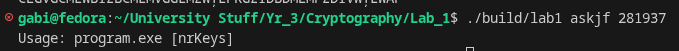
\includegraphics[width=\textwidth]{screenshots/args_incorrect.png}
\caption{Argument-count validation in the existing executable}
\label{fig:arguments}
\end{figure}


Figure~\ref{fig:invalid} demonstrates message retries after punctuation, an emoji, and Hebrew characters. The validator reports only the first unsupported code point in each message. Decoding succeeds for these well-formed Unicode characters; membership validation rejects them because the cipher accepts only the Romanian alphabet and ordinary spaces.

\begin{figure}[htbp]
\centering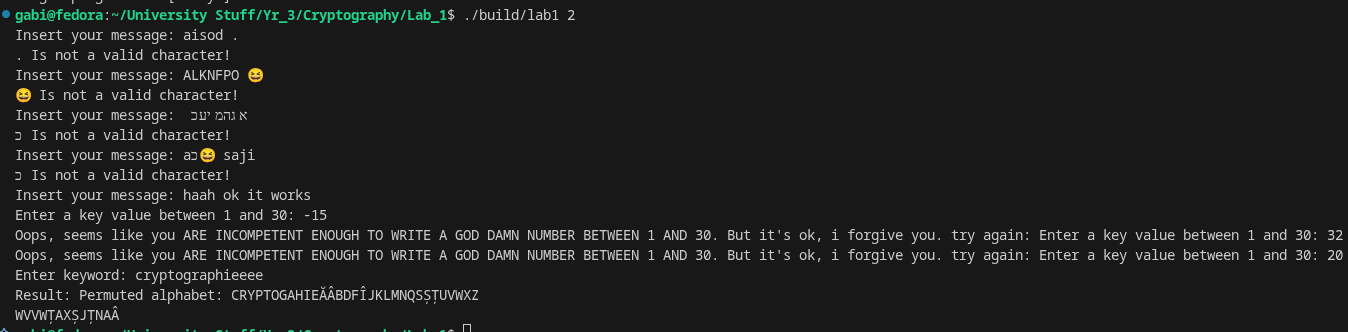
\includegraphics[width=\textwidth]{screenshots/invalids.png}
\caption{Rejected characters and out-of-range shifts, followed by successful encryption}
\label{fig:invalid}
\end{figure}

The accepted message is \texttt{haah ok it works}. The numeric inputs $-15$ and 32 are rejected, and the program requests another key. The accepted key is $k=20$. Using the keyword \texttt{cryptographieeee} then produces \texttt{WVVWȚAXȘJȚNAÂ}. Repeated letters make the substitution visible: the two $A$ letters in the normalized plaintext both become $V$. The screenshots retain the program's original diagnostic wording.

\section{Supplementary verification}
The CMake build completed using the configured C++23 standard and warning flags, including \texttt{-Werror}. The outputs above were reproduced from the compiled program and checked against the supplied screenshots.

To verify functionality that the console does not expose, a temporary C++ harness included the unchanged source with its entry point renamed by the preprocessor. It called both cipher functions directly. This check does not add a decryption menu or constitute an existing project test suite. The calls for the two example ciphertexts are equivalent to:
\begin{cppcode}
caesarCipher(standardCiphertext, 6, true);
caesarPermutationCipher(keywordCiphertext, 8, "UCRAINA", true);
\end{cppcode}
Both returned the same normalized plaintext:
\begin{console}
TRIMITEDOUĂSUTEDEMIIDESOLDAȚISĂCUCEREASCĂMOLDOVA
\end{console}
The harness also encrypted and decrypted all 31 alphabet letters for every allowed shift, once with the standard alphabet and once with the \texttt{UCRAINA} permutation. All 60 full-alphabet round trips passed. Additional checks confirmed the screenshot ciphertexts, the exact keyword alphabet, repeated-keyword-letter handling, cedilla/case normalization, and wraparound.

Encoding checks round-tripped values at the one-, two-, three- and four-byte boundaries, across the scalar-value range. The tested values were \texttt{U+0000}, \texttt{U+007F}, \texttt{U+0080}, \texttt{U+07FF}, \texttt{U+0800}, \texttt{U+D7FF}, \texttt{U+E000}, \texttt{U+FFFF}, \texttt{U+10000}, and \texttt{U+10FFFF}. Mixed text containing Romanian letters, a euro sign, an emoji, and a Hebrew letter also round-tripped through the conversion functions. Eleven malformed UTF-8 inputs tested isolated continuation bytes, truncation, incorrect continuation prefixes, overlong encodings, a surrogate, an out-of-range value, and an invalid leading byte; all were rejected. Encoder checks rejected \texttt{U+D800}, \texttt{U+DFFF}, and \texttt{U+110000}.

Separate executable runs confirmed rejection of a six-letter keyword, the four-letter keyword \texttt{ăâîș} despite its eight UTF-8 bytes, and an internal keyword space. The short-keyword case can be reproduced from the \texttt{Lab\_1} directory with:
\begin{console}
printf 'ABC\n8\nROMANA\n' | ./build/lab1 2
\end{console}
It prints \texttt{Keyword must contain at least 7 characters.} and exits with status 1. These are supplementary execution checks, not additional screenshots supplied with the laboratory.

\section{Scope relative to the assignment}
The source implements both cipher directions, the required alphabet ordering, keyword permutation, custom Unicode conversion, and message/key validation. The submitted screenshots document encryption for both modes and several invalid-input cases. They do not show decryption or a short-keyword error. Decryption was verified at function level above; interactive operation selection remains absent, and invalid keywords terminate instead of being requested again. Character diagnostics identify the rejected character but do not list the entire permitted alphabet. These distinctions describe the current implementation without attributing features to it that belong only to the assignment specification.

\utmconclusions
The laboratory demonstrates that implementing a cipher over a non-ASCII alphabet involves two separate problems: representing characters correctly and transforming their positions correctly. The explicit 31-letter alphabet ensures that modular arithmetic follows the required Romanian encoding. The keyword variant changes that ordering while retaining a reversible substitution.

The custom UTF-8/UTF-32 layer was the most substantial extension of the exercise. Implementing it required identifying byte prefixes, extracting and assembling payload bits, checking sequence boundaries, rejecting overlong encodings and invalid scalar values, and restoring UTF-8 output. It enables code-point-based keyword length checks, predictable Romanian case handling, and diagnostics that preserve an unsupported multibyte character. Supporting all four UTF-8 sequence lengths also separates the general representation layer from the narrower alphabet policy.

The verified round trips confirm the inverse arithmetic for every permitted shift, while the console runs demonstrate normalization and recovery from invalid messages and numeric keys. The standard cipher remains vulnerable to a search over only 30 keys. The keyword variant enlarges the possible substitutions but retains letter frequencies and repeated-letter structure; neither construction provides modern confidentiality. The main learning outcomes are precise text representation, modular arithmetic, validation at multiple layers, and understanding the difference between encoding correctness and cryptographic security.

\chapter*{Source code}
\addcontentsline{toc}{chapter}{Source code}
The C++ implementation and CMake configuration are associated with the laboratory repository:
\begin{center}\url{\repositoryurl}\end{center}
The application is implemented in \path{Lab_1/src/main.cpp}. Its build configuration is stored in \path{Lab_1/CMakeLists.txt}. The report uses the existing UTM LaTeX class; its code excerpts are read directly from the application source at PDF build time.
\begin{thebibliography}{9}
\bibitem{handout} \textit{Laboratory Work No. 1. Caesar Cipher}. Supplied course handout, Tasks 1.1 and 1.2 and report requirements, pp. 1--4.
\bibitem{implementation} Gabriel Balan. \textit{Laboratory Work No. 1: C++ implementation}. Local source \texttt{Lab\_1/src/main.cpp} and \texttt{Lab\_1/CMakeLists.txt}, examined for this report.
\end{thebibliography}
\end{document}
